\chapter{Operating System Layer: In-network Near-Memory Processing}
\label{chap:os}
In the previous chapter, we examined the design of memory management for disaggregated architectures at the service layer. However, integrating general-purpose applications (beyond serverless data analytics) with an external memory service (e.g., Jiffy) often necessitates significant code rewrites to accommodate its API, which may be an undesirable burden for application developers. In this chapter, we shift focus to the potential of embedding memory management functionality directly within the operating system (OS). By enabling the OS to handle memory management transparently, existing data center applications can be seamlessly transitioned to a disaggregated architecture, allowing them to benefit from the high resource utilization and efficiency that such architectures provide.

\section{Background: In-network OS design}

Despite the increased interest in memory disaggregation from both academia~\cite{memdisagg2, memdisagg3, memdisagg4, memdisagg5, memdisagg6, memdisagg1, legoos, infiniswap, fastswap, disagg, disaggfault} and industry~\cite{industry0, industry1, industry2, industry3, industry4, industry5}, memory disaggregation still faces three major challenges. First, remote memory access must have low latency and high throughput, with targets of $10~\mu$s latency and $100$ Gbps bandwidth per compute blade~\cite{legoos, infiniswap, fastswap, disagg}. Second, both compute and memory resources need to scale elastically. Finally, adoption requires support for unmodified applications.

We present \mind, the first memory management system for rack-scale disaggregated memory that addresses these challenges by placing the \mmm within the network fabric, leveraging programmable network switches~\cite{progswitch1, progswitch2}.

%To achieve this, \mind introduces:
%\begin{itemize}
%  \item \textbf{Global Virtual Address Space}: A range-partitioned virtual address space across memory blades to minimize address translation overhead.
%  \item \textbf{Domain-Based Memory Protection}: Decouples permissions from address translation, allowing flexible protection with minimal switch memory overhead.
%  \item \textbf{Directory-Based Cache Coherence}: Adapts MSI coherence~\cite{msi} using switch ASIC multicast to minimize network overhead.
%  \item \textbf{Dynamic Memory Region Sizing}: Adjusts memory region sizes dynamically, balancing performance and storage efficiency.
%\end{itemize}

\begin{table}
    \caption[Parallels between memory \& networking primitives]{\small \textbf{Parallels between memory \& networking primitives.}}
    \label{table:isomorph}
    \centering
    \scriptsize
    \renewcommand{\arraystretch}{1.2}
    \begin{tabular}{p{3cm} p{1cm}p{3cm}}
      \hline
      \textbf{Virtual Memory} &$\Longleftrightarrow$ &\textbf{Networking} \\\hline\hline
      Memory allocation&&IP assignment\\
      Address translation &&IP forwarding\\
      Memory protection  &&Access control\\
      Cache invalidations &&Multicast\\
      \hline
    \end{tabular}
\end{table}


\begin{figure*}[!t]
\centering
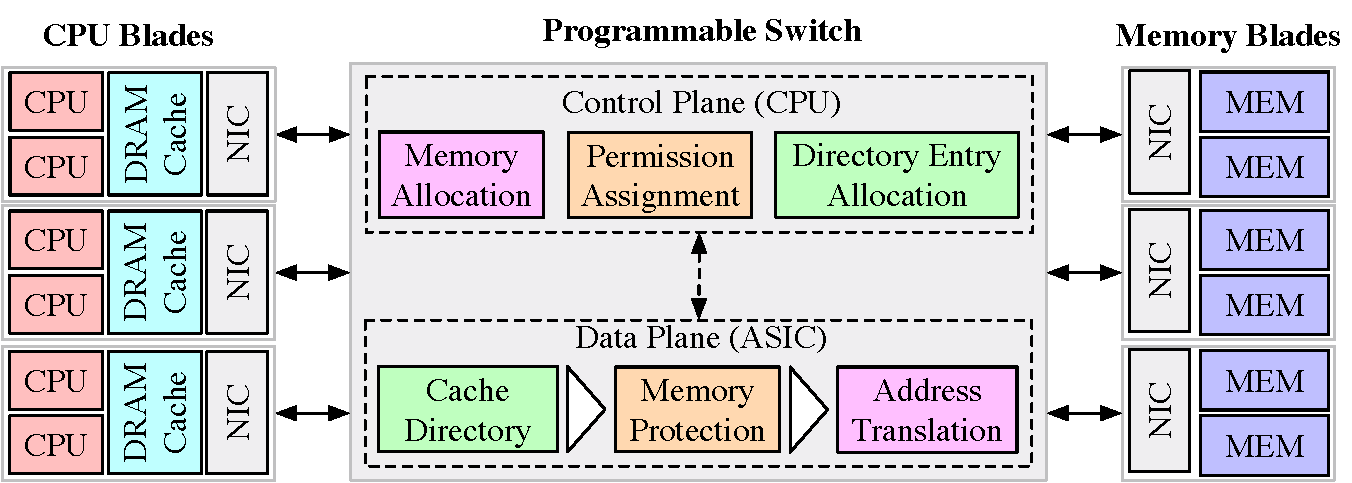
\includegraphics[width=0.55\textwidth]{fig/mind/design}\hspace{3em}
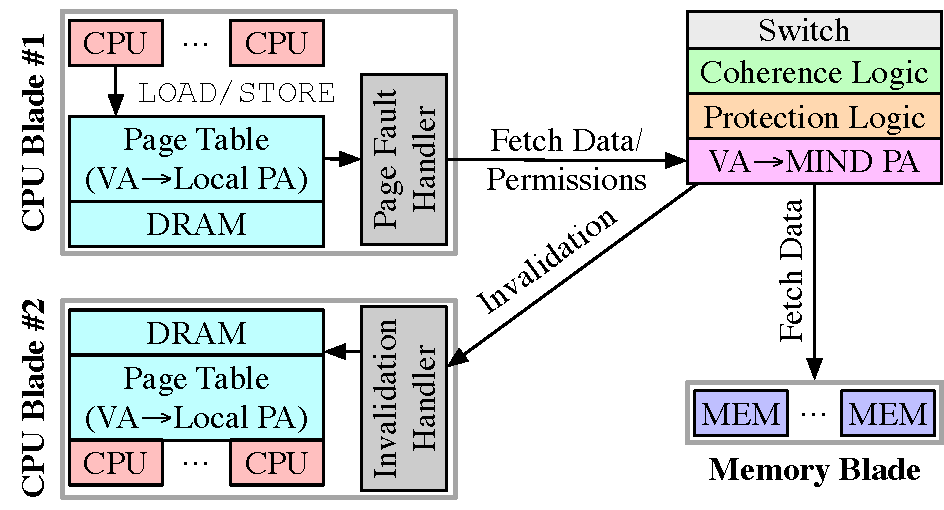
\includegraphics[width=0.35\textwidth]{fig/mind/data_flow}%\vspace{-1em}
\vspace{-0.5em}
\caption[High-level \mind architecture and data flow for memory accesses in \mind]{\textbf{(left) High-level \mind architecture, and, (right) data flow for memory accesses in \mind.}}
\label{fig:system_diagram}
\end{figure*}

\mind places memory management \textit{in the network fabric} for three key reasons: (1) its central location and global view allow direct memory access without metadata coherence, (2) modern programmable network switches~\cite{progswitch1} execute at line rate, which is a good target for implementing the memory management logic, and (3) placing cache coherence logic in the network reduces latency and bandwidth overhead. 

\mind exposes a \textit{transparent virtual memory} abstraction to applications, similar to traditional OSes. It intercepts memory allocations at CPU blades and performs memory operations via RDMA, leveraging a switch-based MMU for cache coherence. Memory blades store pages and serve RDMA requests directly, enabling true hardware disaggregation. Figure~\ref{fig:system_diagram}(left) shows an overview of \mind's design, while Figure\ref{fig:system_diagram}~(right) illustrates its memory access flow. CPU blades run user processes and use local DRAM as a cache. Memory allocations and deallocations are intercepted and forwarded to the switch control plane, which manages allocations and permissions. All memory operations are handled by the CPU cache, with virtual addresses translated locally. If a page is not cached, a page fault triggers RDMA to fetch it from memory blades. Coherence updates also trigger page faults, handled by the switch.Since the CPU blade lacks memory metadata, RDMA requests only use virtual addresses. The switch data plane intercepts them, handling cache coherence, permission checks, and address translation. If no cache holds the page, it forwards the request to the correct memory blade. \mind relies on one-sided RDMA, eliminating the need for CPUs on memory blades, moving towards full hardware disaggregation.

